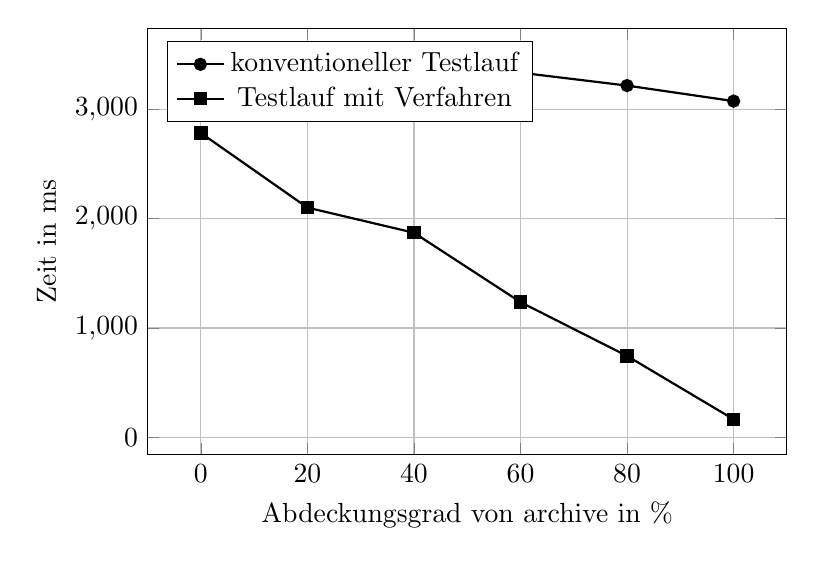
\begin{tikzpicture}
    \begin{axis}[
        width=0.8\textwidth,
        height=7cm,
        xlabel={Abdeckungsgrad von archive in \%},
        ylabel={Zeit in ms},
        grid=major,
        legend pos=north west
    ]
    \addplot[
        thick,
        mark=*,
    ] coordinates {
        (0, 3237.9)
        (20, 3417.2)
        (40, 3410.0)
        (60, 3335.6)
        (80, 3217.6)
        (100, 3075.6)
    };
    \addlegendentry{konventioneller Testlauf}
    \addplot[
        thick,
        mark=square*,
    ] coordinates {
        (0, 2783.8)
        (20, 2101.1)
        (40, 1871.0)
        (60, 1236.2)
        (80, 743.7)
        (100, 164.0)
    };
    \addlegendentry{Testlauf mit Verfahren}
    \end{axis}
\end{tikzpicture}
